% this file is called up by thesis.tex
% content in this file will be fed into the main document

%: ----------------------- name of chapter  -------------------------
\chapter{The ONE simulator}\label{simulatore} % top level followed by section, subsection


%: ----------------------- paths to graphics ------------------------

% change according to folder and file names
\graphicspath{{2-simulatore/img/}}


%: ----------------------- contents from here ------------------------
The simulation environment chosen for our simulations is The ONE (Opportunistic Network Environment) version 1.4.1\footnote{The ONE simulator \href{http://www.netlab.tkk.fi/tutkimus/dtn/theone/}{http://www.netlab.tkk.fi/tutkimus/dtn/theone/}}, described in \cite{articoloONE}. This simulation environment written in Java is completely configurable and is able to simulate completely the behaviour of nodes in the simulations, including movement, connections and to give a visual feedback about all these factors using its GUI. A more interesting feature, for our purposes, is the capability of emulate message routing using different routing protocols.
\\
 
To emulate nodes movement, the ONE can take in input traces from real-world measurements, from external mobility generators or it can generate movement patterns using synthetic mobility model generators. Differences between several available mobility are explained in Section \ref{movimento}. Either mobility models that routing protocols are managed like independent modules, which are dynamically loaded depending on what set in configuration files. This allow a relatively easy implementation of new mobility models and routing protocols in the simulator.
\\

The simulator finally allow to save data of interest from the completed simulations into report files. This reports are created using modules dynamically loaded in the same way to what happens with movement and routing modules.
\\

\section{Configuration}
\label{configurazioneONE}
A single simulation is set, before running, using configuration files which describe the simulated environment, from the simulation length to number of nodes emulating people in the simulated environment. Configuration files are text-based files that contain parameters about the simulation, user interface, event generation, and reporting modules. All these parameters are loaded before the beginning of simulations and are used to adjust details about the behaviour of loaded modules.
\\

Many of the simulation parameters are configurable sepa-
rately for each node group but groups can also share a set of param-
eters and only alter the parameters that are specific for the group.
The configuration system also allows defining of an array of val-
ues for each parameter hence enabling easy sensitivity analysis: in
batch runs, a different value is chosen for each run so that large
amounts of permutations are explored.

Inside configuration files, parameters are saved as key-value pairs and syntax for most of the
variables is:

\begin{center}
\textit{Namespace.key = value}
\end{center}

Namespace defines the part of the simulation environment where the setting has effect on. Many, but not all, namespaces are equal to the class name where they are read. This convention is especially followed by movement models, report modules and routing modules, so also created new modules should follow it.
\\

To make human-readability and configuration easier, numerical values can use suffixes kilo (k), mega (M) o giga (G), with \textquotedblleft .\textquotedblright as decimal separator. Boolean parameters accept \textquotedblleft true\textquotedblright
 or \textquotedblleft 1\textquotedblright , \textquotedblleft false\textquotedblright or \textquotedblleft 0 \textquotedblright .
\\
 
Comments can be inserted in setting files can contain comments too with \textquotedblleft
\#\textquotedblright character. Rest of the line is skipped when the settings are read.
\\

Every simulation can be set using several configuration files, to divide parameters into different categories, e.g. a file can contain scenario parameters, like maps, streets and districts, another file can contain parameters used to configure nodes, another file can contain reports configuration and so on. First configuration file read, if exists, is always \textquotedblleft default\_settings.txt\textquotedblright. Other configuration files given as parameter can define more settings or override some (or even all) settings in the previous files. The idea is that you can define in the earlier files all the settings that are common for
all the simulations and run different simulations changing parameters only in latests configuration files.
\\

The basic agents in the simulator are called nodes. A node models a mobile endpoint capable of acting as a store-carry-forward router (e.g., a pedestrian, car or tram with the required hardware). Nodes in the simulation world are divided into groups, each one configured with different capabilities. Inside a group, every node has the same characteristics, which are radio interface, persistent storage, movement, energy consumption and message routing protocol. It is possible to configure some of these capabilities as common for all groups, avoiding to set them individually for each group. Changing some configuration value between a group and another, allow to get heterogeneity between the behaviour of nodes in simulated scenario.
\\

In configuration files is also possible to provide array of settings for every parameter. This allows to run large amounts of different simulations using only single configuration file. Every simulation will be different from the previous and this is very useful to gather reports about different aspects in a common scenario.
\\ Syntax for these configuration parameters is

\begin{center}
\textit{Namespace.key = [run1_value; run2_value; run3_value; etc]}
\end{center}

Some parameters, finally, accept a file path as value and this can be either an absolute or relative path. These parameters are used for maps, nodes paths or events to be loaded by event generators modules.

\section{Simulation outputs}
The way to follow the progress of simulations is the GUI present in the ONE. In main window, shown in Fig.\ref{Schermata-ONE}, is possible to observe movements of nodes acting in the simulation and view details about one of them by selecting it from the list of active nodes. For every node is possible to get informations about active connections, messages carried and other details. In the main window is also present a log panel updated with a textual description of events generated in the current simulation. These events can be filtered allowing to see only logs related to one kind of events e.g. new connections, creation of messages or massage exchanges.
\\
\begin{figure}[htpb]
  \begin{center}
    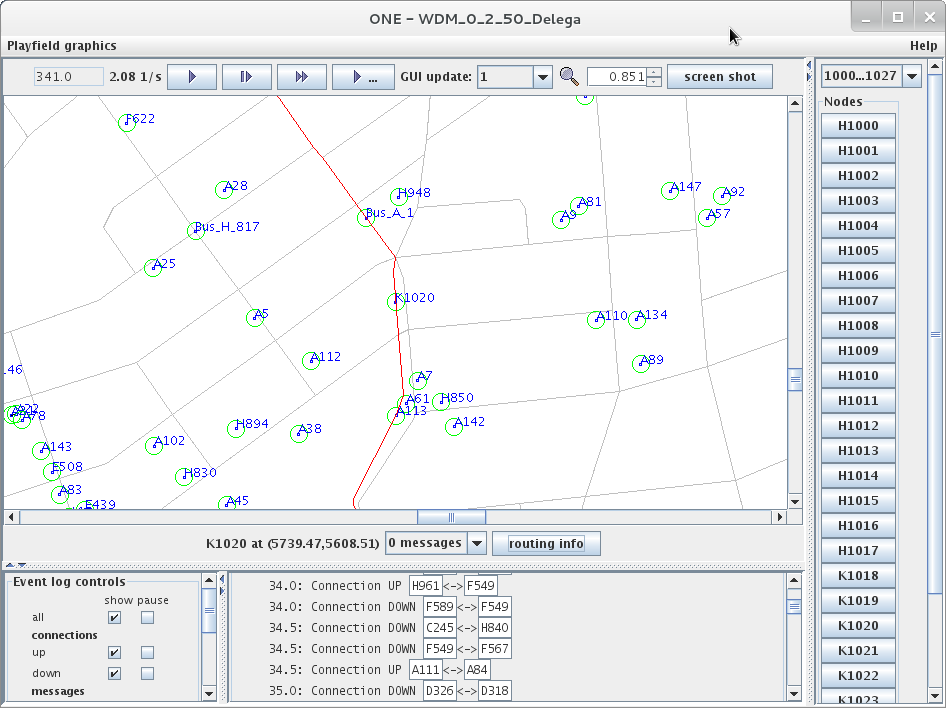
\includegraphics[scale=0.9]{2-simulatore/img/Schermata-ONE.png}
    \caption[Main window]{Main Window of the ONE}    
    \label{Schermata-ONE}
  \end{center}
\end{figure}
%\figuremacro{Schermata-ONE}{Schermata Principale}{La schermata principale del simulatore ONE}{}

Selecting a node is also possible to follow its movements inside the simulated world map, with the path to its next destination highlighted in the graphical visualization of the map. A pop-up window, shown in Fig. \ref{Routing-Info}, can be invoked to get advanced informations about the state of that node.
\\

\begin{figure}[htpb]
  \begin{center}
    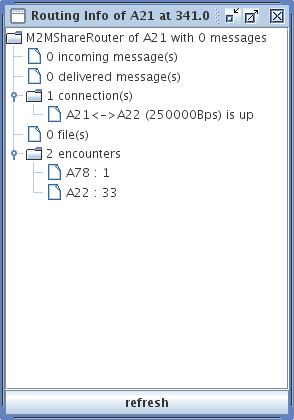
\includegraphics[scale=0.6]{2-simulatore/img/Routing-Info.png}
    \caption[Routing Info]{Main Window of the ONE}    
    \label{Routing-Info}
  \end{center}
\end{figure}
%\figuremacro{Routing-Info}{Routing Info}{Un esempio di finestra in cui sono presenti i dettagli relativi allo stato di un nodo}{}

The map representation is configurable and the user can adjust the zoom level, simulation speed and it's possible to add an image as background, e.g. using a road map or a satellite photo of the interested area.
\\

The other way to follow the progress of simulations is to read generated reports, at the end of the simulation. Each report is generated by its related module and these modules, like movement and routing modules, are dynamically loaded at the beginning of the simulation according to what set in configuration files. To use report files is particularly useful when doing simulations in batch, without using the GUI and analysing resulting reports when all the set of simulations is complete. In batch mode is useful the possibility of define arrays of values for parameters in configuration files. These allow to set differences in configuration between the different runs of the batch. When the batch is executed, the ONE would run all the simulations, reading for each of them the correct configuration parameters, and saving the generated reports into different files for each simulation run.
\\

Several report modules can be active during one single simulation. Output of these modules are report files, which typically are text-based files in which are saved statistical and log data gathered during the simulation. These data can be further analysed when the simulation has ended. In the ONE version 1.4.1, the simulator has some ready to use report modules which allow to create reports related to:

\begin{description}
\item[messages,] e.g. number of created messages, delivery times, expired messages, etc..
\item[contacts,] which can show contact and inter-contact time between the nodes, or the number of contacts during the simulation
\item[connections,] which can show changes in connections status
\end{description}

Report modules are handled by the simulator like other modules and this allow to easily implement and add new report modules to the simulator, to gather needed data from simulations.


\section{Simulation execution}
\label{esecuzioneONE}
It can be interesting to explain in detail how a single simulation is run by the simulator. Let's see what steps are performed for each run.
\\

The first step done is configuration loading. The simulator read from configuration files values assigned to simulation parameters. Configuration files path are passed as arguments to the ONE launch command. When a configuration file is read, values contained are used to initialize or overwrite the value of some variables in simulation environment. If some parameters value is not set in configuration files, default values are used and an exception is thrown if a default value was not present for that parameter.
\\

When the simulation is configured, the creation of the simulated scenario begins. The scenario contains all active entities in the simulation, i.e. nodes, report generators or event generators, and passive entities, i.e. maps which composes the simulated world. In this phase all nodes are created and initialized according to the configuration loaded. Every node contains a router implementing one routing protocol, uses one movement model and has some \textit{listener} associated used to catch events and generate reports.
\\

Quando tutte le entità necessarie all'esecuzione sono stati create e configurate, si passa all'esecuzione vera e propria.
Questa consiste nel ripetere l'aggiornamento dello stato del mondo, chiamando un metodo \textit{update()}, e incrementare il valore del tempo simulato fino al raggiungimento di un tempo impostato come fine simulazione. L'incremento temporale che viene effettuato ad ogni aggiornamento è impostato nei files di configurazione (con il parametro \textit{Scenario.updateInterval}), espresso in secondi, ed influenza i vari modelli di movimento dei nodi. La prima operazione svolta durante l'\textit{update()} del mondo simulato è lo spostamento dei vari nodi, che avviene a seconda del modello di movimento adottato dal nodo e dell'incremento temporale applicato. Ad esempio un nodo che simula un automobilista si sposterà maggiormente rispetto ad uno che simula un pedone, a parità di intervallo di tempo simulato. Come vedremo nella sezione \ref{movimento} relativa ai modelli di movimento, questi possono essere anche molto complessi e simulare diversi comportamenti a seconda delle configurazioni adottate.
\\

Una volta effettuato il movimento, per ogni nodo viene aggiornato lo stato delle connessioni e del router simulato. Per ogni interfaccia di rete disponibile viene quindi aggiornato lo stato a seconda che lo spostamento abbia comportato una caduta della connessione o abbia permesso di entrare nel raggio di comunicazione di un interfaccia di rete relativa ad un altro nodo. Ogni qualvolta lo stato di una connessione cambia, vengono avvisati i \textit{listeners} interessati, per la generazione di report, e viene aggiornata la visualizzazione grafica della connessione, se attiva, come si può vedere, ad esempio, in Figura \ref{connessioni}.
\\
\figuremacro{connessioni}{connessioni}{Un esempio di connessioni tra nodi tratto dalla finestra principale di ONE. Nella parte sinistra dell'immagine si può notare la connessione attiva, mentre nella parte a destra i due nodi non sono più l'uno nel raggio di comunicazione dell'altro, indicato dal cerchio verde attorno al nodo.}{}

L'ultima parte dell'aggiornamento relativo allo stato di un nodo riguarda l'aggiornamento del router. Questo è fortemente dipendente dal protocollo di routing implementato ed è proprio nell'esecuzione del metodo \textit{update()} relativo al router che si svolgono le azioni caratteristiche di un protocollo rispetto ad un altro.

\section{Casualità}
come viene introdotta della casualità nelle varie simulazioni

\section{Limitazioni}
\label{limitazioniONE}
non più in basso del livello di routing
simulazione temporale discreta
mancanza di simulazione di un file system

\section{The map}
\label{mappaONE}
qua ci va la descrizione della mappa con la divisione in distretti e magari un'immagine delle rotte dei bus e del modello di movimento
% ---------------------------------------------------------------------------
%: ----------------------- end of thesis sub-document ------------------------
% ---------------------------------------------------------------------------

